\section{Intermediate Representations}
\label{bg:sec:intermediate}

Intermediate representations (IRs) are data structures designed to be
independent of the machine architecture and source language.  They are often
invented with the intention to ease program analysis and optimization in mind,
by abstracting information from the original program that are irrelevant to our
objectives.  In this section, we introduce several categories of existing IRs,
and delve deeper into the advantages and disadvantages of each.

\subsection{Static Single Assignment Form and Control-Flow Graph}
\label{bg:sub:ssa_cfg}

Traditionally, \emph{static single assignment} (SSA) form~\cite{alpern88,
rau92} together with \emph{control-flow graph} (CFG) are used to represent
data- and control-flow of a program~\cite{cytron91}, because they are more
favorable program representations on which optimization passes can be
implemented, when compared to the original HLL or the output language.  SSA can
be advantageous in implementing conventional optimization techniques, \eg~code
motion~\cite{cytron86}, removing redundant computations~\cite{rosen88},
and constant propagation~\cite{cytron91}.  Because the LLVM intermediate
representation (LLVM IR)~\cite{llvm_ir} is based on SSA and CFG, and is
commonly used in many HLS tools such as LegUp~\cite{legup}, we introduce SSA
and CFG by compiling the dot-product example in Figure~\ref{bg:lst:dotprod}
into as shown in Figure~\ref{bg:lst:dotprod_ll}.
\begin{figure}[ht]
    \centering
    \begin{lstlisting}[language=LLVM]
define float @dotprod(
    float* nocapture readonly %A,
    float* nocapture readonly %B) #0
{
; <label>:0
  br label %2

; <label>:1         ; preds = %2
  ret float %8

; <label>:2         ; preds = %2, %0
  %i.02 = phi i32 [ 0, %0 ], [ %9, %2 ]
  %d.01 = phi float [ 0.000000e+00, %0 ], [ %8, %2 ]
  %3 = getelementptr inbounds float, float* %A, i32 %i.02
  %4 = load float, float* %3, align 4, !tbaa !2
  %5 = getelementptr inbounds float, float* %B, i32 %i.02
  %6 = load float, float* %5, align 4, !tbaa !2
  %7 = fmul float %4, %6
  %8 = fadd float %d.01, %7
  %9 = add nuw nsw i32 %i.02, 1
  %exitcond = icmp eq i32 %9, 1024
  br i1 %exitcond, label %1, label %2
}
    \end{lstlisting}
    \caption{%
        The compiled and optimized LLVM IR output from the dot-product example
        in Figure~\ref{bg:lst:dotprod}.
    }\label{bg:lst:dotprod_ll}
\end{figure}

The LLVM IR of our example function consists of parts that are known as
\emph{basic blocks} (BB), each BB in turn often contains a label that
uniquely identifies the BB, a list of LLVM IR statements in SSA form
without any branches, \ie~the statements are executed sequentially, and a
terminator instruction, which is typically a branch instruction that leads
the control-flow to a different BB, by referencing a BB label, or a function
return.

The LLVM framework implicitly constructs a CFG from the IR code, which is a
directed graph representing the control-flow of a program.  The vertices in
the CFG constitute BBs, while the edges indicate the control-flow directions
(\ie~branches to other BBs), often with predicate attributes to determine
whether the branch is taken.  For instance, we consider the first line of third
BB in Figure~\ref{bg:lst:dotprod_ll}:
\begin{lstlisting}[language=LLVM, basicstyle=\tt]
    ; <label>:2     ; preds = %2 %0
\end{lstlisting}\vspace{-16.5pt}
which indicates it has a label value $2$ and the control-flow coming to this
BB is from either BB2 or BB0, here we use BB$n$ as a shorthand denoting a
BB labelled $n$.  Additionally, this BB ends with the branch terminator
instruction:
\begin{lstlisting}[language=LLVM, basicstyle=\tt]
    br i1 %exitcond, label %1, label %2
\end{lstlisting}\vspace{-16.5pt}
This instruction directs the control-flow to BB1 or BB2, and the variable
\verb|%exitcond| in the terminator instruction decides which branch is taken.
Finally, the complete CFG is shown in Figure~\ref{bg:fig:dotprod_cfg}.  It is
noteworthy that BB2 has two edges that leads to either \verb|BB1| or \verb|BB2|
itself.  If \verb|%exitcond| evaluates to false (\textbf{ff}), then another
iteration of BB2 will commence, otherwise (\textbf{tt}) the exit condition is
satisfied and will lead the control-flow to \verb|BB1|.
\begin{figure}[ht]
    \centering
    \tikzstyle{block} = [
        draw, fill=white, rectangle, minimum height=2em, minimum width=3em
    ]
    \tikzstyle{tmp} = [coordinate]
    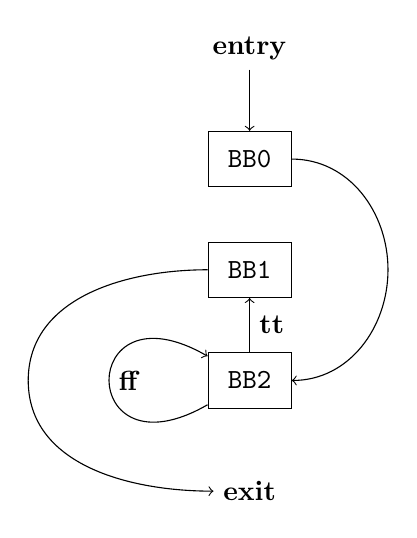
\begin{tikzpicture}
        \node [] (entry) {\textbf{entry}};
        \node [block, below of=entry, node distance=4em] (bb0) {\texttt{BB0}};
        \node [block, below of=bb0, node distance=4em] (bb1) {\texttt{BB1}};
        \node [block, below of=bb1, node distance=4em] (bb2) {\texttt{BB2}};
        \node [tmp, right of=bb1, node distance=5em] (bb1tr) {};
        \node [tmp, left of=bb2, node distance=8em] (bb2tl) {};
        \node [tmp, right of=bb2, node distance=8em] (bb2tr) {};
        \node [below of=bb2, node distance=4em] (exit) {\textbf{exit}};
        \draw [->] (entry) -- (bb0);
        \draw [- ] (bb0)    to[out=0, in=90]    (bb1tr);
        \draw [->] (bb1tr)  to[out=-90, in=0]   (bb2);
        \draw [- ] (bb1)    to[out=180, in=90]  (bb2tl);
        \draw [->] (bb2tl)  to[out=-90, in=180] (exit);
        \draw [->] (bb2) -- node[auto, swap]{\textbf{tt}} (bb1);
        \draw [->] (bb2) to[out=-150, in=150, loop]
            node[auto, swap]{\textbf{ff}} (bb2);
    \end{tikzpicture}
    \caption{The CFG of the LLVM IR code in Figure~\ref{bg:lst:dotprod_ll}.
    }\label{bg:fig:dotprod_cfg}
\end{figure}

Each BB contains sequential computations that are represented by SSA
instructions.  The SSA form describes the operations in the original
program, such that each variable in it is assigned exactly one value.

The sequence of instructions that assigns to \verb|%3|-\verb|%9| in
Figure~\ref{bg:lst:dotprod_ll} carries out most of the computations in the
program.  It starts by reading \verb|A[i]| and \verb|B[i]|, multiplying them
together, then add the result with \verb|d| to form a new variable, and
finally, the iteration value is accumulated by $1$.  It may seem unusual that
both the accumulated sum of products and the iteration value are not assigned
to \verb|d| and \verb|i| respectively.  We can imagine two BBs, one initializes
\verb|d| and \verb|i| to zeros, the other accumulates these two variables in
a loop.  As all variables must be assigned once only, one of the BBs should
use different names for these two variables.  When the control-flow of these
two BBs join, we must introduce a way to read from the variables that are
assigned in the two BBs in the succeeding BB\@.  A new instruction, called the
$\phi$-function is therefore defined for our purpose.  The $\phi$-function
accepts two variable names as its inputs, and produce the value of either
variable as its output, determined by which preceding BB the control-flow came
from.  For example, in LLVM IR, the instruction:
\begin{lstlisting}[language=LLVM, basicstyle=\tt]
    %d.01 = phi float [ 0.000000e+00, %0 ], [ %8, %2 ]
\end{lstlisting}\vspace{-16.5pt}
shows that if the control-flow originated from BB0, then a constant zero is
returned, otherwise the control-flow had to come from BB2 and the value of
\verb|%8| is used instead.

The rationale of SSA is that we can abstract away anti- and output dependences
by never assigning to the same variable twice, while only true data-flow
dependences remain.  Anti-dependence is a dependence relation when a read
operation must precede a write to the same variable, and output dependence is
when two writes refer to the same location.  By removing these dependences
and deferring the analysis of them, certain program optimization analyses
can run much more efficiently.  Analyses that may benefit from this include
scheduling~\cite{rau94}, and liveness analysis (figure out the life time
of variables to reduce register requirements)~\cite{cytron91}, detecting
opportunities of parallelism~\cite{cytron87}, and finding equivalent parts in
the program~\cite{alpern88}.

In a cyclic CFG, the control-flow could potentially revisit a BB, and
instructions in this BB will inevitably assign a different value to the
same variable, which forms anti- and output dependences, which could have a
detrimental effect on efficient loop pipelining in some computing machines.  An
alternative IR, the \emph{dynamic single assignment} (DSA) form~\cite{rau92}
can therefore be used in place of the SSA to address this issue.  The DSA
defines a linear sequence of virtual registers for each variable, such that
every time the variable is assigned in a dynamic execution path, a new virtual
register is used.

\subsubsection{Alternatives to SSA and CFG}

There are a number of alternative IRs that are similar in construction to
the SSA and CFG approach in LLVM IR\@.  For instance, the data-dependence
graph~\cite{rau94} introduced in Section~\ref{bg:sub:sdc} are designed
for the purpose of capturing data-flow dependences in polyhedral methods.
\emph{Data-flow graph} (DFG) is a popular alternative to SSA, which is often
a directed acyclic graph (DAG) that do not contain cyclic paths.  In general,
a DFG's vertices are input, output and operation nodes, and the edges capture
the dependences between these nodes.  Both of them, however, generally do
not preserve enough information for us to reconstruct a program from the
graph itself.  A group of data structures, known as \emph{control/data flow
graphs} (CDFGs)~\cite{orailoglu86}, is commonly used to represent programs in
HLS tools, \eg~SPARK~\cite{gupta04}.  A CDFG resembles a CFG such as the one
used in LLVM IR, but in lieu of using sequential instructions in SSA form in
graph vertices, each vertex contains a \emph{data-flow graph} (DFG), where no
SSA temporary variables are used and data-flow dependences can by explicitly
identified by edges.


\subsection{Equality Saturation}
\label{bg:sub:equality_saturation}

The IRs we discussed above are all used to analyze and transform the underlying
program structure, so as to produce a new representation of the optimized
program.  In a conventional optimizing compiler, program optimization is
often carried out in a sequence of transformation passes, where each pass
accepts a program, often written in a certain IR, and produces an optimized
program in the IR\@.  The traditional practice is to always apply these
optimization phases in a fixed order, but a good ordering of these phases
is crucial to achieve a good optimized result, and the optimal ordering
varies across applications being compiled~\cite{almagor04}.  The process of
finding the optimal ordering is known as the \emph{phase-ordering problem},
which is in general undecidable~\cite{touati06} and hence is a difficult
problem.  Moreover, programs running CPUs or GPUs usually care only about
their throughput, in contrast, designs on FPGAs concern us with additional
objectives besides run time, such as power consumption and resource utilization
that impact the quality of synthesized circuit.  Multiple designs that
trade-off these objectives could exist, and which design to choose relies
on the specifics of the use case.  It is therefore sensible to explore the
design space by optimizing multiple objectives simultaneously.  For the
above reasons, it is desirable to have an IR and the associated optimization
procedures to efficiently discover equivalent structures that lead to different
implementations of the original program.

In software, a novel approach called \emph{equality saturation} is proposed
in~\cite{tate09} to find multiple possible optimized variants of the original
program, and subsequently deal with the phase-ordering problem.  It creates
a new graph-based IR, \emph{program expression graph} (PEG), to encode the
effects of executing the program.

To begin, we review the structure of the PEG, by considering a simple loop
example in Figure~\ref{bg:fig:factorial}.  By understanding how the PEG can
be evaluated for the output values, we can interpret how the PEG captures the
control- and data-flow information of the program.  PEGs, similar to arithmetic
expressions expressed in a tree structure, can be evaluated in a bottom-up
fashion, by recursively propagating computed values from the leave nodes to the
root of the tree.  However, unlike arithmetic expressions which are acyclic,
edges in PEGs may form cycles to express loops in the original program.
\begin{figure}[ht]
    \newsavebox{\factlstbox}
    \begin{lrbox}{\factlstbox}
    \begin{lstlisting}
int x = 1;
int y = 1;
while (y <= 10)
{
    x = y * x;
    y = y + 1;
}
    \end{lstlisting}
    \end{lrbox}
    \centering
    \subfloat[The original program.]{%
        \begin{minipage}{0.4\textwidth}
            \usebox{\factlstbox}
        \end{minipage}\label{bg:lst:factorial_c}
    }
    \subfloat[The resulting PEG.]{%
        \begin{minipage}{0.5\textwidth}
            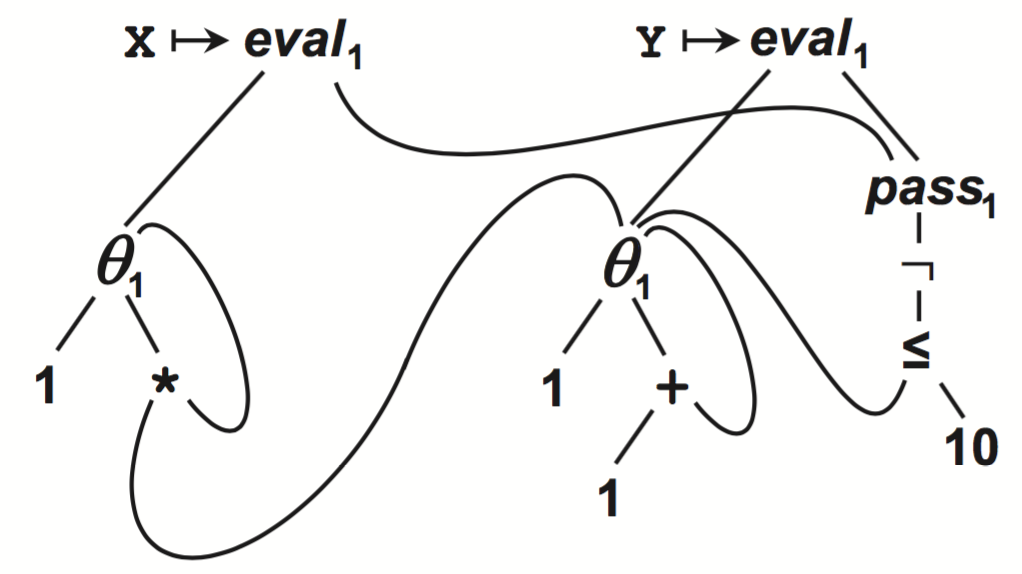
\includegraphics[width=\textwidth]{bg/fig/factorial_peg.png}
        \end{minipage}\label{bg:fig:factorial_peg}
    }
    \caption{%
        A simple loop which computes the factorial of 10, and the resulting
        PEG\@.  This example and its PEG, showing computations that lead to the
        final \texttt{x} and \texttt{y}, is taken from~\cite{tate09}.
    }\label{bg:fig:factorial}
\end{figure}

\subsubsection{Data-Flow Nodes}

All loops in the PEG are formed by $\theta$ nodes, which is used in the
following form:
\begin{center}
    \vspace{-16.5pt}
    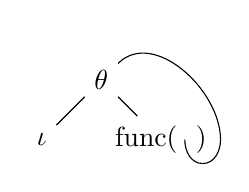
\begin{tikzpicture}
        \node (theta) at (0, 0) {$\theta$};
        \node (init) at (-5ex, -5ex) {$\iota$};
        \node (func) at (5ex, -5ex) {$\mathrm{func}(~~)$};
        \node[coordinate] (input) at (7ex, -5ex) {};
        \node[coordinate] (mid1) at (8.5ex, -7ex) {};
        \node[coordinate] (mid2) at (10ex, -5ex) {};
        \draw[-] (theta) -- (init);
        \draw[-] (theta) -- (func);
        \draw[-] (input) to[out=-90, in=180] (mid1);
        \draw[-] (mid1) to[out=0, in=-90] (mid2);
        \draw[-] (mid2) to[out=90, in=45] (theta);
    \end{tikzpicture}
    \vspace{-16.5pt}
\end{center}
where it accepts two child graphs, $\iota$ and $\mathrm{func}$, and
$\mathrm{func}$ further takes the $\theta$ node as one of its inputs to
form a complete cycle.  Evaluating a $\theta$ node produces a list of
values computed iteratively by the node's subgraph.  The first value in the
list, is the computed result of $\iota$, which we name $i$, and values in
the rest of the sequence are iteratively computed by $\mathrm{func}$.  In
functional programming, this is similar to iteratively computing the fixpoint
$\mathbf{fix}\,F$ of an initial list $[i]$, which is defined as:
\begin{equation}
    \mathbf{fix}\,F ([i]) = \lim_{n \to \infty} F^n ([i]),
    \quad\text{where~}
    F(v) = \mathrm{prepend}\left(
        i, \mathrm{map}\left( \mathrm{func}, v \right)
    \right)
\end{equation}
here, $\mathrm{map}(\mathrm{func}, v)$ applies the subgraph computation
$\mathrm{func}$ to all elements in the list $v$, and $\mathrm{prepend}(i,
v^\prime)$ prepends the element $i$ to the list $v^\prime$.

For example, the following subgraph in Figure~\ref{bg:fig:factorial_peg}
evaluates to the sequence $[1, 2, 3, 4, \mathellipsis]$:
\begin{center}
    \vspace{-16.5pt}
    \begin{tikzpicture}
        \node (theta) at (0, 0) {$\theta_1$};
        \node (init) at (-5ex, -5ex) {$1$};
        \node (add) at (5ex, -5ex) {$+$};
        \node (one) at (0, -10ex) {$1$};
        \node[coordinate] (mid) at (8ex, -5ex) {};
        \draw[-] (theta) -- (init);
        \draw[-] (theta) -- (add);
        \draw[-] (add) -- (one);
        \draw[-] (add) to[out=-45, in=-90] (mid);
        \draw[-] (mid) to[out=90, in=45] (theta);
    \end{tikzpicture}
    \vspace{-16.5pt}
\end{center}

It is noteworthy that $\theta$ nodes may have subscripts.  For instance,
in Figure~\ref{bg:fig:factorial_peg}, both nodes $\theta_1$ share the same
subscript $1$.  This is used to indicate that the two sequences produced
by both $\theta$ nodes iterate simultaneously, \ie~they share the same
iteration count so that a new value for \verb|x| can be computed as we update
\verb|y|.  Therefore, the $\theta_1$ node in the left of this figure produces
a sequence of the factorials of $[1, 2, 3, \mathellipsis]$, \ie~$[1, 2, 6, 24,
\mathellipsis]$.

Computation nodes, such as arithmetic $+$ and boolean operators $\leq$ and
$\neg$ in Figure~\ref{bg:fig:factorial_peg}, operates on a list of values, by
performing the computation on each value in the list.

For instance, the $\leq$ node accepts two inputs, the sequence $[1, 2, 3,
\mathellipsis]$ derived earlier, and a scalar $10$, computes the result of $x
\leq 10$ for each element $x$ in the sequence, and finally produces the list,
where $\truelit$ and $\falselit$ respectively denote true and false boolean
values:
\begin{equation}
    [
        \truelit, \truelit, \truelit, \truelit, \truelit,
        \truelit, \truelit, \truelit, \truelit, \truelit,
        \falselit, \falselit, \falselit, \mathellipsis
    ].
\end{equation}
The subsequent $\neg$ node then negates all elements in the list:
\begin{equation}
    [
        \falselit, \falselit, \falselit, \falselit, \falselit,
        \falselit, \falselit, \falselit, \falselit, \falselit,
        \truelit, \truelit, \truelit, \mathellipsis
    ].
    \label{bg:eq:bool_seq}
\end{equation}

\subsubsection{Control-Flow Nodes}

The $\theta$ node encodes an infinite sequence of computed values, whereas
the output value of the program is a scalar.  By further representing
control-flow information in PEG, it becomes possible to refer to a
single value in this sequence, as the output of the program.  To do so,
Tate~\etal~\cite{tate09} further introduce $\mathrm{pass}$ and $\mathrm{eval}$
nodes.  The $\mathrm{pass}$ node finds the first true ($\truelit$) value
in a sequence of boolean values, and returns the index of this value, and
$\mathrm{eval}$ takes two child nodes, where the first node evaluates to a list
$v$ of values, and the second is an scalar $n$ used to select a scalar value
from $l$, as the output of this node.

To illustrate, the $\mathrm{pass}_1$ node finds the first $\truelit$ in the
list~\eqref{bg:eq:bool_seq}, $11$.  The $\mathrm{eval}$ node of the output
variable \verb|y| subsequently fetches the $11$-th item from the list $[1, 2,
3, 4, \mathellipsis]$ we produced earlier, which is $11$.  Similarly we can
apply the same process to find that the output \verb|x| is $10!\,$, \ie~the
factorial of 10.

By using $\mathrm{pass}$ and $\mathrm{eval}$ nodes to represent the
control-flow in an algebraic fashion, and mixing data- and control-flows
together in the graphical representation, PEGs provide us with greater
opportunities to optimize data-flow across control-flow boundaries and vice
versa.  Simple equivalence rules can be defined for these nodes algebraically.
For instance, arithmetic operators can be distributed over $\theta$ and
$\mathrm{eval}$, \eg~$\mathrm{eval}(j, k) + i \equiv \mathrm{eval}(j + i, k)$.
Complex transformations can therefore be deductively constructed from these
simple equivalence rules.

\subsubsection{Equivalence Finding}

By applying transformation passes to the PEG, their approach detects the
incremental modifications, and append these changes to the original PEG\@.  The
new changes, represented as extra structures in the PEG, are linked to their
corresponding equivalent nodes by equivalence edges.  These edges indicate a
pair of subgraphs are equivalent, forming a PEG with equivalent structures,
or named E-PEG, that could capture multiple PEGs in the same structure.  The
resulting E-PEG is similar to the one in Figure~\ref{bg:fig:epeg}, where dashed
edges indicate equivalences.  It is notable that each edge allows a binary
choice, therefore the number of PEGs can be represented in an E-PEG could be
exponential in the number of equivalence edges.
\begin{figure}[ht]
    \centering
    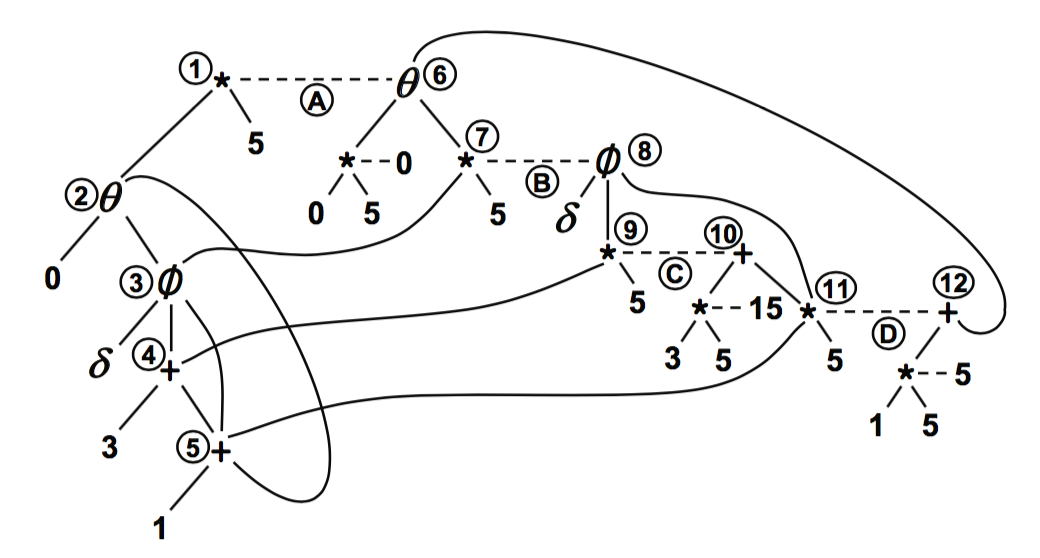
\includegraphics[width=0.8\linewidth]{bg/fig/epeg.png}
    \caption{An simple E-PEG example, taken from~\cite{tate09}.
    }\label{bg:fig:epeg}
\end{figure}

By repeatedly applying all possible passes to the E-PEG, this graph will
eventually saturate, \ie~no more equivalent structure can be added to the graph
because all possible equivalences are now discovered.  This process and the
resulting E-PEG is more space-time efficient than enumerating all possible PEGs
along the path, because E-PEG encourages sharing common subgraphs, even across
equivalent edges.  This saturated graph can always be produced regardless of in
what order we apply the passes, hence preventing the phase-ordering problem.
Furthermore, E-PEG defers the decision of whether an optimization should be
committed until we have reached full saturation, allowing the global optima to
be discovered.  In contrast, because each optimization pass in a conventional
compiler is performed once, the compilers must make the decision to commit
changes immediately after applying the optimization, which consequently often
results in local optima.
